\plainFrame{%
    \begin{multicols}{2}
        \centering
        {\Large Environment}
        \begin{tikzpicture}
            \pause
            \node (roads) {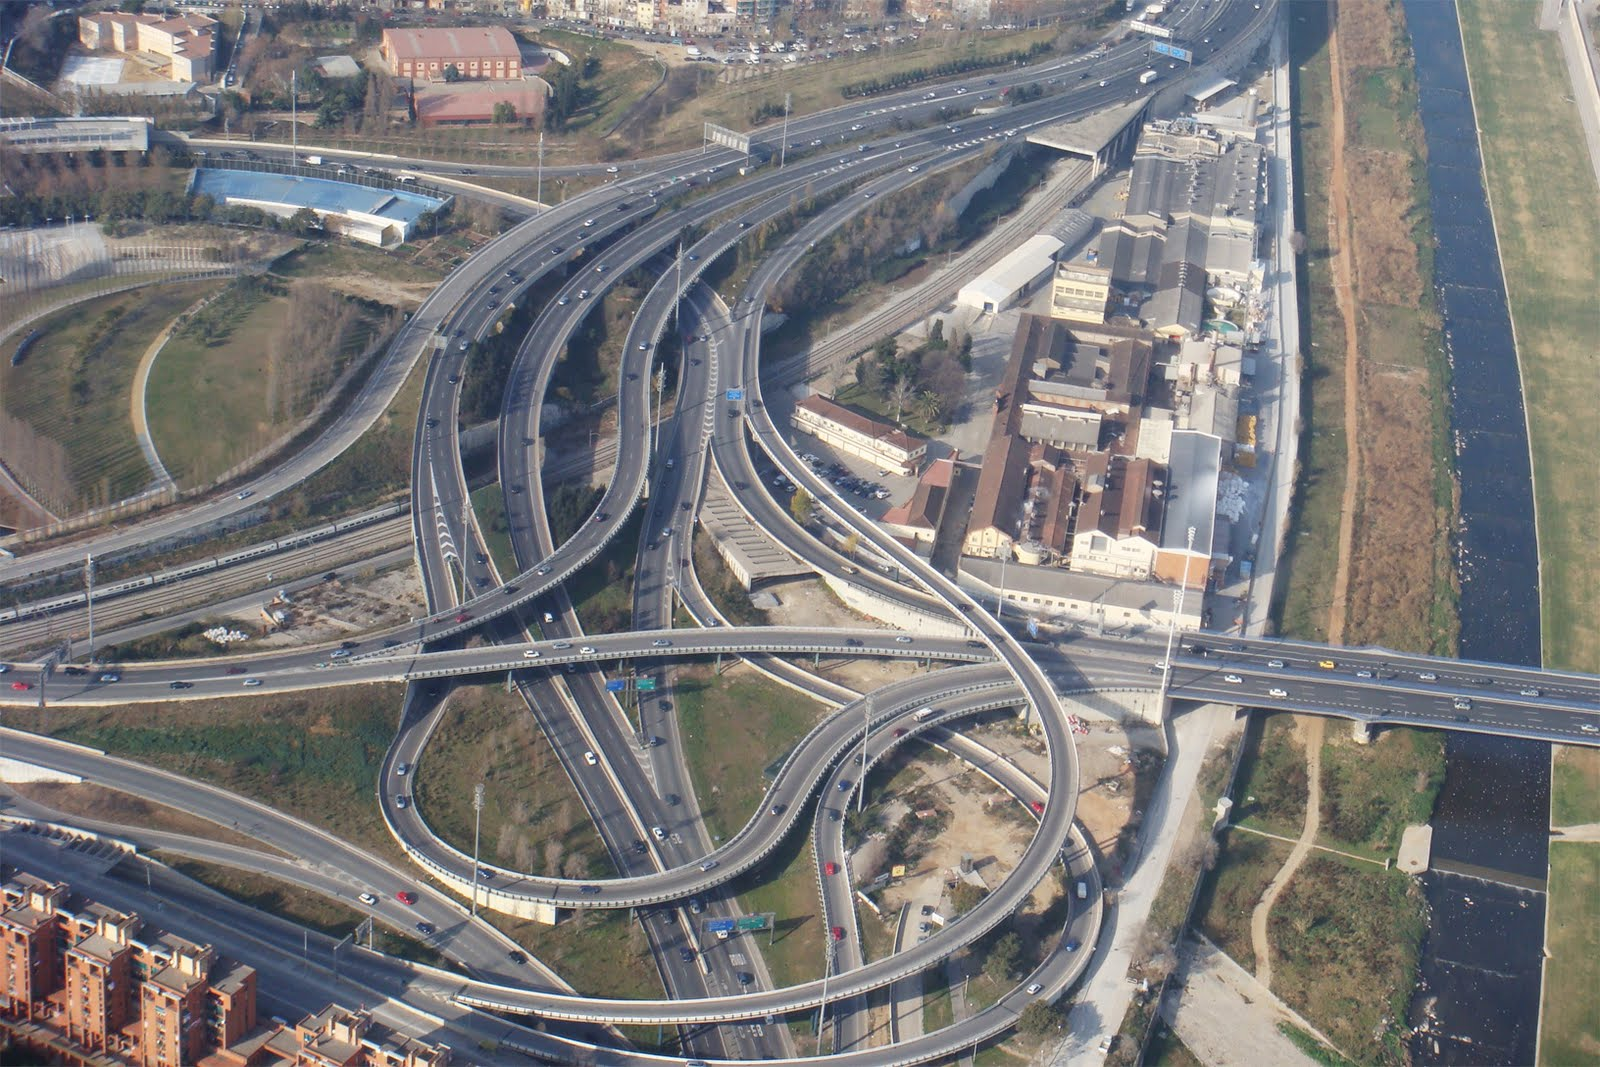
\includegraphics[width=\linewidth]{media/Crazy_Road_Network.jpg}};
            \pause
            \node (obstacles) at (roads.south) {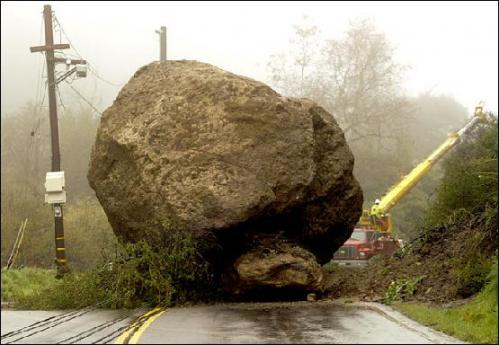
\includegraphics[width=\linewidth]{media/obstacle-on-your-road.jpg}};
        \end{tikzpicture}
        \vfill\null%
        \columnbreak%
        \onslide<1->{{\Large Test Setup}}
        \onslide<4->{
            \begin{tikzpicture}
                \pause
                \node (car) {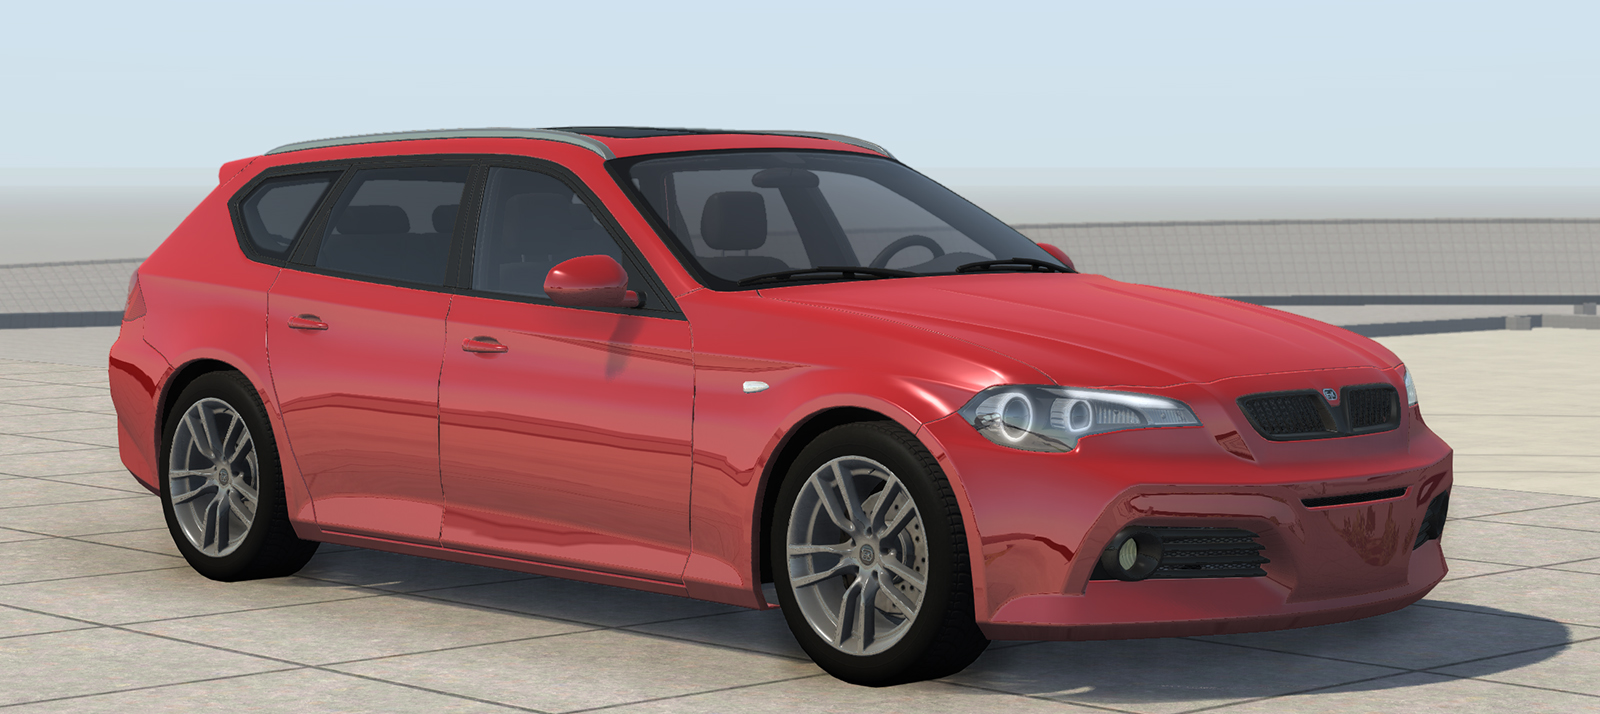
\includegraphics[width=\linewidth]{media/etk800thread.jpg}};
                \pause
                % FIXME Should I mention movement?
                \node (movement) at (car.south) {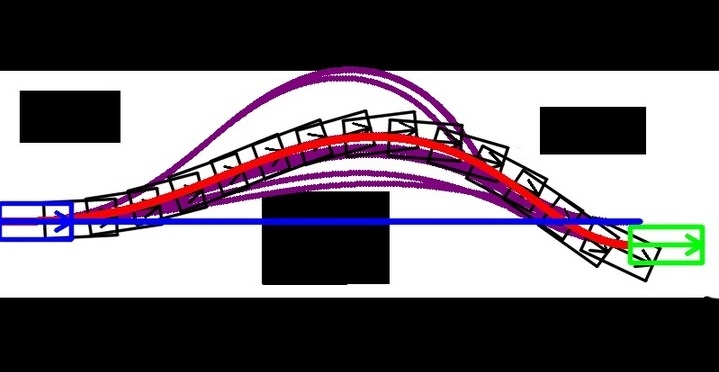
\includegraphics[width=\linewidth]{media/nlp.jpg}};
                \pause
                \node (criteria) at (movement.south) {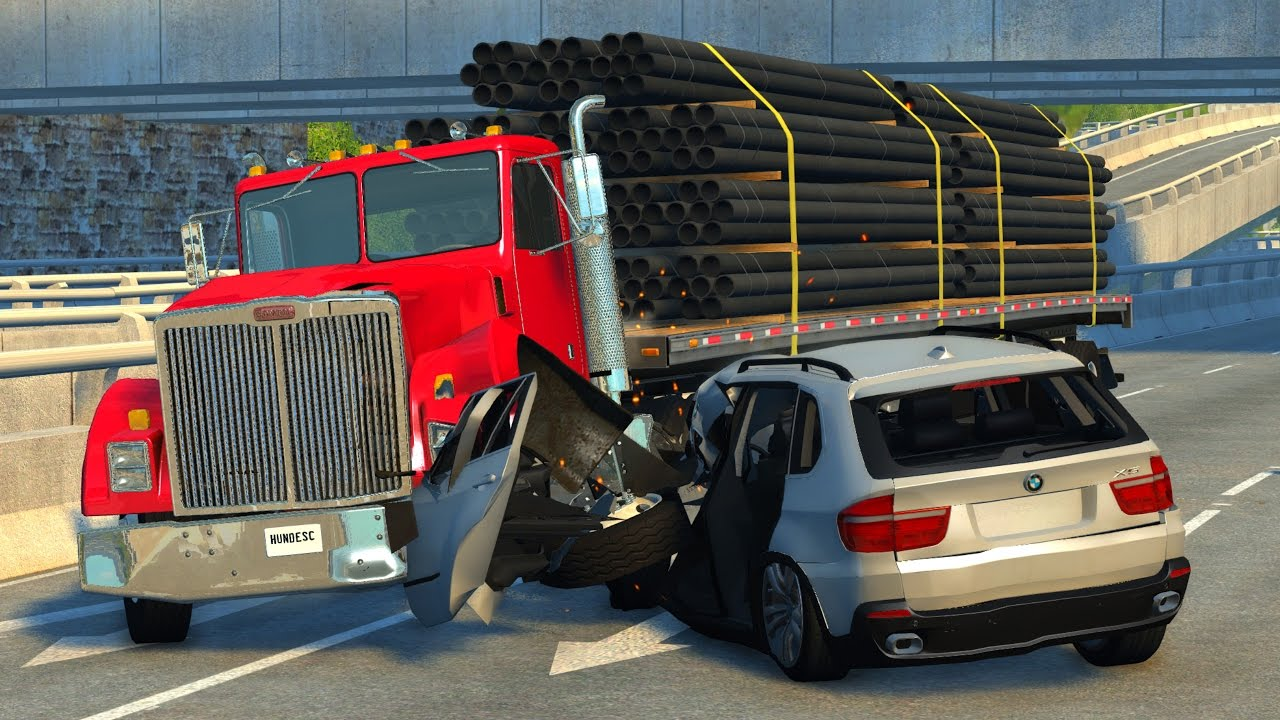
\includegraphics[width=\linewidth]{media/maxresdefault.jpg}};
                \pause
                \node (offroad) at (car) {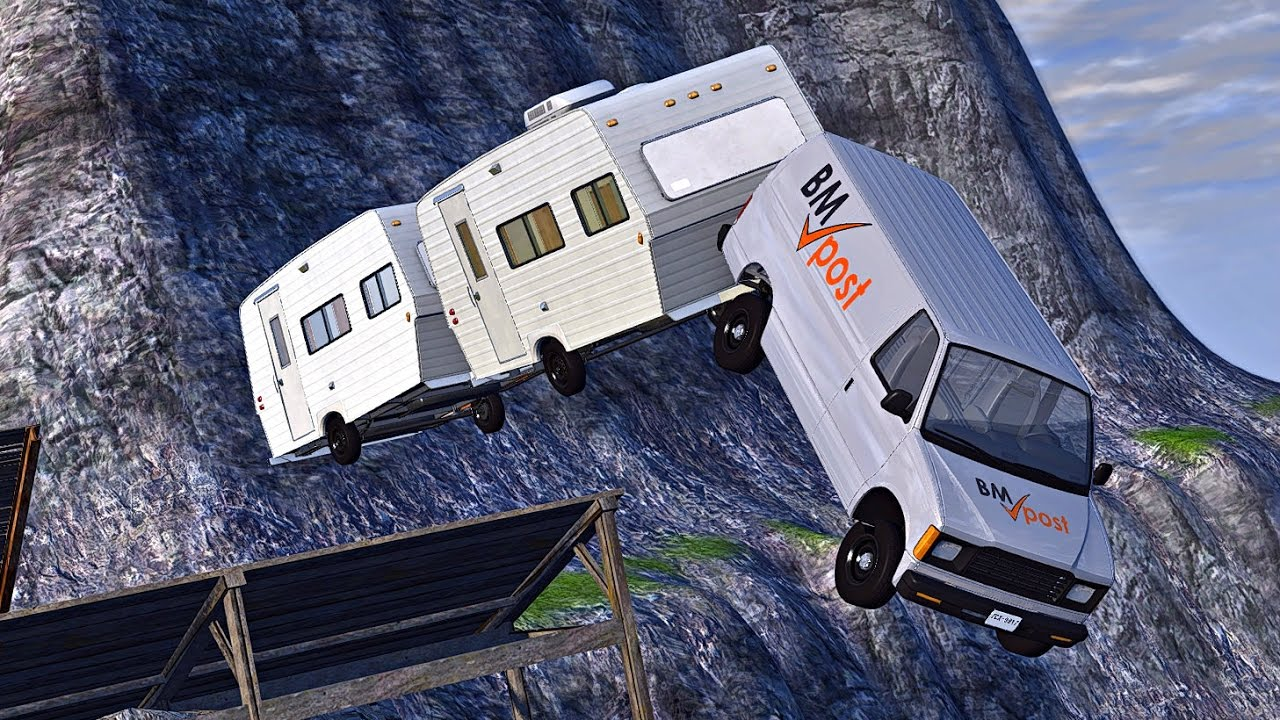
\includegraphics[width=\linewidth]{media/maxresdefault2.jpg}};
                \pause
                \node (finish) at (offroad.south) {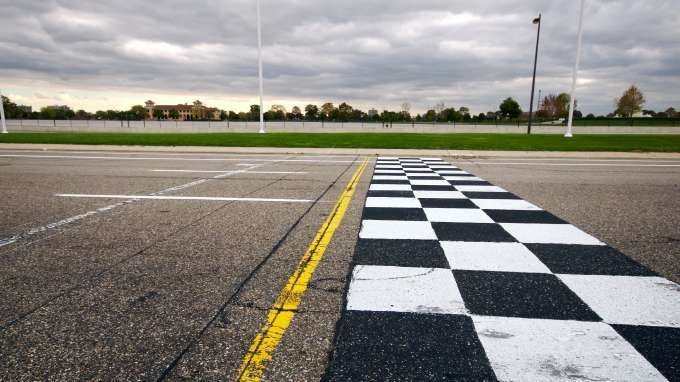
\includegraphics[width=\linewidth]{media/1349.jpg}};
            \end{tikzpicture}
        }
    \end{multicols}
    \subsectionBox<1->{colorFormalize!50}
}

